    \documentclass[11pt]{article}

\usepackage{fullpage}
\usepackage{xcolor}
\usepackage{amsmath}
\usepackage{hyperref}
\usepackage{graphicx}
\usepackage[ruled,vlined,linesnumbered]{algorithm2e}


\pdfpagewidth 8.5in
\pdfpageheight 11in 



\oddsidemargin 0in
\evensidemargin 0in


\newtheorem{claim}{Claim}
\newtheorem{definition}{Definition}
\newtheorem{theorem}{Theorem}
\newtheorem{lemma}{Lemma}
\newtheorem{observation}{Observation}
\newtheorem{question}{Question}
\newtheorem{problem}{Problem}

\newcommand{\re}{{\mathbb{R}}}
\newcommand{\floor}[1]{\lfloor {#1} \rfloor}
\newcommand{\ceil}[1]{\lceil {#1} \rceil}
\newcommand{\paren}[1]{\left( {#1} \right)}


\begin{document}
	
\begin{center}
\Large{\textbf{CS 330, Fall 2020, Homework 10 \\
Due Wednesday, November 18, 2020, 11:59 pm Eastern Time}}
\end{center}

\begin{center}
    \color{teal}
   Student: Justin DiEmmanuele \\
    Collaborators: Shilpen Patel, George Padavick, Matthew Gilgo
\end{center}



\begin{enumerate}
\item
{\bf Cell tower problem}

The company operating the cell towers is at it again. This time they need to install towers along a long country road connecting two cities.  Help them find the best location for the towers! Each installed tower covers an area of 5 miles' radius (i.e. 5 miles on either side of the tower). There needs to be cell coverage along the entire road.  There is infrastructure to install a tower at every milestone along the road. The total distance between the cities is $n$ miles. (You are allowed to place a tower in either city.)  The cost of installing towers varies by location. The costs of the different locations are given to you in an array \texttt{cost[\ ]} of the length $n+1$. (The costs are positive numbers.) You need to find  a set of building sites such that the entire road has cell coverage and the total cost is minimized. 



\begin{enumerate}
\item Observe that it is possible that the minimum cost solution consists of stretches of road that are covered by multiple towers. Prove however, that in any \emph{optimal} solution, each stretch is covered by at most $2$ towers.

    \begin{itemize}
        \color{teal}
        \item Suppose we have a stretch of road that is covered by three towers.
            One possibility, is that two of the towers are in the same 
            position. In this case it is clear that one of the towers is 
            redundant because the removal of one does not change the stretch
            of road covered. 
        \item The second, less clear case, is where all three of the towers are
            in different locations. Again, at least one point along the road
            is covered by three towers. If this were the case, one tower would
            be the left most tower and one would be the right most. The middle 
            tower will always be redundant as it will not stretch as far left 
            as the left most tower and also will not stretch as far right as the
            right most tower. Since there is one space where all three towers 
            cover, we know that the left and right most towers can span the 
            entire covered interval on their own. This means the middle tower 
            will always be redundant. This extends to any number of towers 
            larger than 2.
    \end{itemize}

    \newpage
 \item Consider a greedy algorithm where we add locations to our solution set one at a time. We consider the stretches of road (the road between two neighboring tower locations) in increasing order of distance from the first city. Each time we encounter a so far uncovered road stretch $r_i$ (that is between miles $i-1$ to $i$), we will add a tower location $j$  that (1.) covers $r_i$ (2.) has the best cost-coverage ratio. That is, we choose a location $j$ such that the relative cost $\frac{\texttt{cost[j]}}{\texttt{additional\ miles}}$ of every additional mile covered by this tower is minimized. 
     
 Show an example where this algorithm fails. 

     \begin{itemize}
         \color{teal}
     \item Drawn in the following figure is a counterexample to the stated 
         rule. The tower we are focused on here is tower b. Assuming towers 
         a and c are in the lowest-cost positions they could be in, the lowest
         cost position for b to have complete coverage over the interval is 
         clearly where it is placed with a cost of 3. This would give a value 
         of $\frac{3}{6}$ since the tower has a cost of 3 and covers 6 more 
         miles than what was previously covered. Notice that if we place tower 
         b at location 15 instead, the cost is 4 and 10 more miles are covered.
         this gives a relative cost of $\frac{4}{10}$ which is lower than 
         that of the present location, yet the present location has a lower 
         cost of 3. The proposed rule would not work in this case.

             \begin{figure}[htpb]
                 \centering
                 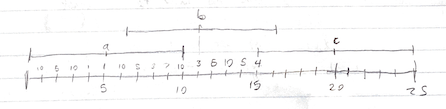
\includegraphics[width=0.8\textwidth]{1b.png}
                 \caption{\color{teal}Counterexample}
                 \label{fig:Counterexample1b}
             \end{figure}
     \end{itemize}
 
    
 \newpage
    \item\label{part:0} Here is the pseudocode for a memoized algorithm to find the \emph{minimum cost} of locations. (Note that it does not give you the actual set of locations.) \\
    
    \begin{algorithm}[H]\label{algo:towers}
        \caption{DPMinCostTowers(\texttt{cost}, $n$)}
        $M \gets $ empty array of length $n$\;
        \For{$i=0 \ldots n$ }{
            $M[i] \gets$ \{some appropriate formula to be defined by you\}\;
        }
        \Return $M[n]$\;
    \end{algorithm}
      
 
    
    What  does the entry \texttt{M[i]} contain (that is, state the subproblem for which it provides a solution)? 
    \begin{itemize}
        \color{teal}
    \item $M[i]$ contains the cheapest solution in which there is a tower at
        position $i$. This is represented by the following formula:
        \[
            M[i] = cost[i] + min \{M[i-10],\ldots, M[i-1]\} 
        .\] 
    \end{itemize}

    Write the recursive formula to compute \texttt{M[i]} in line 3 of the algorithm. (Write the formula only, no need for explanation. )

    \begin{algorithm}[H]\label{algo:towers}
        \color{teal}
        \caption{DPMinCostTowers(\texttt{cost}, $n$)}
        $M \gets $ empty array of length $n$\;
        \For{$i=0 \ldots n$ }{
            \If {$i \le  5$} {
                $M[i] = cost[i]$\;
            }
            \Else {
                $M[i] \gets cost[i] + 
                min\left([M[max(n + i, 0)] \text{ for } i \text{ in } range(-10, 0)]\right) $\;
            }
        }
        \Return $M[n]$\;
    \end{algorithm}

    \color{teal}
    The algorithm essentially implements the formula above but taking into 
    consideration the base cases and possible out of bounds errors when 
    accessing arrays.
    \color{black}
      
 
    

    \item Write an algorithm that takes the table $M$ filled in by Algorithm~\ref{algo:towers} and returns a list of the locations where towers should be built.     

\end{enumerate}

\item {\bf Game tournament}

You are participating in an online gaming tournament. The tournament consists of $n$  competitions. You are eligible to participate in any of them. However, you can only be in one competition at a time, there can be no overlap between the tournaments you enter. Sadly, you'll have to make a choice in which competitions you participate. As an input to this problem you will be given an array \texttt{start[\ ]} of length $n$  containing the start time of each competition, and another array \texttt{duration[\ ]} with the duration of each game. You may assume that the games are indexed $0$ through $n-1$ in increasing order of their start times. 

Since you play for the pure enjoyment of the game, you don't care about your placement in any of the competitions.  Your goal is to pick games so that you {\bf maximize} the time that you spend playing. (If you start a game, you have to finish it.) 
\begin{enumerate}
    \item What algorithm from class could be used to solve this problem? How would you transform the inputs to this problem into the ones needed for the algorithm from class? Make sure you understand how that algorithm works before proceeding. 
      
        \begin{itemize}
            \color{teal}
            \item Weighted interval scheduling in which the weights are the 
                duration of each game.
        \end{itemize}
\item\label{part:2} Due to the large number of entries, the tournament organizers have decided to limit the number of competitions each player can enter to $k$ (so the input now consists of the arrays \texttt{start} and \texttt{duration}, and the number $k$). Your goal is to find a set of at most $k$ tournaments that do not overlap, and whose total duration is as long as possible. Design a polynomial-time dynamic programming algorithm for the problem. Please organize your answer as follows: 

\begin{enumerate}
    
\item Define the set of subproblems that your algorithm will solve. (For example, for the Knapsack problem, the subproblems were: ``for each $i \in \{1,...,n\}$ and $w \in \{1,...,W,\}$: compute the maximum value one can obtain by using only items 1 to $i$ and a knapsack with capacity $w$.") 

[\textit{Hint:} Consider having one subproblem for each $i\in \{1,...,n\}$ and $j \in \{1,...,k\}$. Think carefully about the order in which to consider the tournaments.]

\item How many such subproblems are there?


\item Suppose we create a table $M$ to store the value of the subproblems we solve. Write a recursive formula to compute \texttt{M[i,j]} in terms of other entries of $M$ (that is, the solutions to smaller subproblems). 
(Be mindful to include the base cases.)

\item Explain briefly why your formula is correct. (This explanation is really the proof of correctness for your algorithm.)



\item Write pseudocode for your algorithm (it should fill the memoization table and find the optimal subset of tournaments).

 \item What is the asymptotic running time of your algorithm? (Only write the $\Theta$  formula, no proof needed.)


\end{enumerate}

\end{enumerate}


\end{enumerate}

\end{document}
